\documentclass{standalone}

%Drawing
\usepackage{tikz}
\tikzset{>=latex}
\usetikzlibrary{calc}

%Notation
\usepackage{physics}

% Colors
\definecolor{blue1}{rgb}{0.0, 0.33, 0.71}
\definecolor{blue2}{rgb}{0.29, 0.59, 0.82}

%Newcommand

%Newcommand  
%%Midline Label 
\newcommand{\midlinelabel}[3]%
{    
	\node (midlabel) at ($ (#1)!0.52!(#2) $) {#3};    
	\draw[<-,thick] (#1) --  (midlabel);    
	\draw[->,thick] (midlabel) -- (#2); 
}

\begin{document}
	
	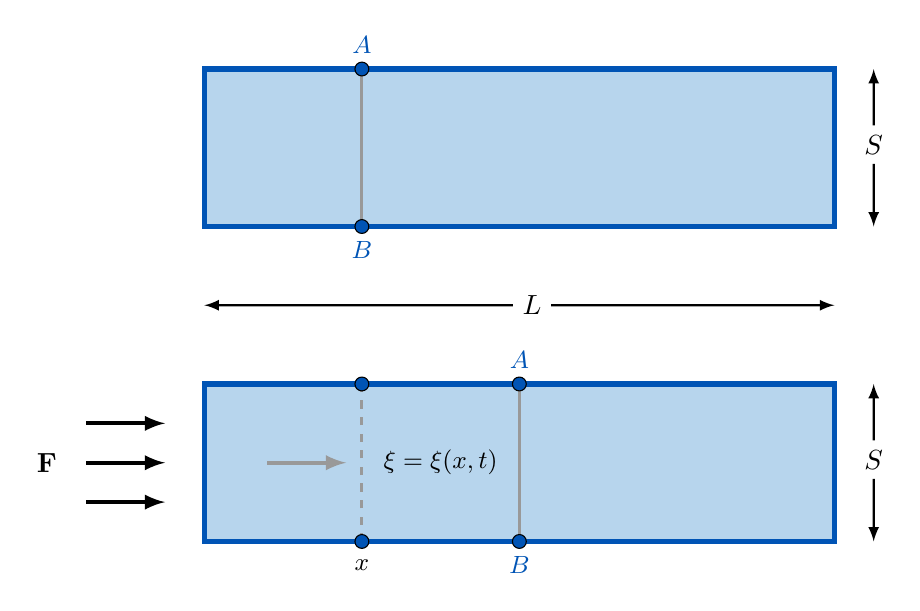
\begin{tikzpicture}
		% Grid
%		\draw[line width = 0.05] (0,0) grid (12,12);

		% Bottom Rectangle
		\draw[line width = 2, blue1, fill = blue2!40] (3,1) rectangle (11,3);
		
		% Upper Rectangle
		\draw[shift = {(0,4)}, line width = 2, blue1, fill = blue2!40] (3,1) rectangle (11,3);
		
		% Gray Lines
		%% Bottom
		\draw[line width = 1.5, black!40, ->] (3.8,2) -- +(1,0);
		\draw[line width = 1, black!40, dashed] (5,1) -- +(0,2);
		\draw[line width = 1, black!40] (7,1) -- +(0,2);	
		%% Top
		\draw[line width = 1, black!40] (5,5) -- +(0,2);
		
		% Points 
		%% A and B
		%%% Bottom
		\foreach \x in {0,2}
		{
			\draw[shift = {(0,\x)}, fill=blue1] (7,1) circle (2.5pt);
		}
		%%% Top
		\foreach \x in {0,2}
		{
			\draw[shift = {(0,\x)}, fill=blue1] (5,5) circle (2.5pt);
		}
		%% Bottom Points Above x
		\foreach \x in {0,2}
		{
			\draw[shift = {(0,\x)}, fill=blue1] (5,1) circle (2.5pt);
		}
		
		% Nodes
		\node at (5,0.7) {\small$x$};
		\node at (1,2) {$\vb{F}$};
		\node[blue1] at (7,0.7) {\small$B$};	
		\node[blue1] at (7,3.3) {\small$A$};	
		\node at (6,2) {\small$\xi = \xi(x,t)$};
		\node[blue1] at (5,4.7) {\small$B$};	
		\node[blue1] at (5,7.3) {\small$A$};	

		% L line
		\midlinelabel{3,4}{11,4}{$L$}
		
		% Force Vectors
		\foreach \x in {0,1,2}
		{
			\draw[shift = {(0,0.5*\x)}, line width = 1.5, ->] (1.5,1.5) -- ++(1,0);
		}
		
		% S Lines
		\midlinelabel{11.5,1}{11.5,3}{$S$}
		\midlinelabel{11.5,5}{11.5,7}{$S$}
	\end{tikzpicture}
	
\end{document}
